\chapter{Estudo de Caso: Atividade 1} \label{Chap:AppendixLesson}

\section{Atividade 1: Plano de Aula}\label{section:atividade1_planoaula}

%\textbf{TEMA:} Trigonometria no Triângulo Retângulo

%\textbf{OBJETIVO GERAL:} Revisar alguns conceitos estudados em anos anteriores relacionados ao triângulo retângulo de modo a possibilitar a introdução de conceitos de relações trigonométricas no círculo trigonométrico.

%\textbf{OBJETIVOS ESPECÍFICOS:}
%\begin{enumerate}
%	\item 
%\end{enumerate}

\begin{table}[htbp]
	\begin{tabularx}{\textwidth}{|l|X|}
	\hline
	\multicolumn{2}{|c|}{\cellcolor[HTML]{C0C0C0}\textbf{TEMA}} \\ \hline
	\multicolumn{2}{|l|}{Trigonometria no Triângulo Retângulo} \\ \hline
	\multicolumn{2}{|c|}{\cellcolor[HTML]{C0C0C0}\textbf{OBJETIVOS}} \\ \hline
	\textbf{GERAL} & Revisar alguns conceitos estudados em anos anteriores relacionados ao triângulo retângulo de modo a possibilitar a introdução de conceitos de relações trigonométricas no círculo trigonométrico.\\ \hline
	\multicolumn{1}{|l|}{\textbf{ESPECÍFICOS}} & \multicolumn{1}{l|}{\begin{tabular}[c]{@{}l@{}}- Introduzir conceitos de básicos de trigonometria\\ - Recordar conceitos básicos de relações trigonométricas no triângulo\\ retângulo\end{tabular}} \\ \hline
	\multicolumn{2}{|c|}{\cellcolor[HTML]{C0C0C0}\textbf{CONTEÚDO}} \\ \hline
	\multicolumn{2}{|l|}{\begin{tabular}[c]{@{}l@{}}Conceito de trigonometria, triângulo retângulo, semelhança de triângulos, catetos, hipotenusa,\\ teorema de Pitágoras, relações trigonométricas do triângulo retângulo (seno, cosseno, tangente)\end{tabular}} \\ \hline
	\multicolumn{2}{|c|}{\cellcolor[HTML]{C0C0C0}\textbf{METODOLOGIA DO ENSINO}} \\ \hline
	\multicolumn{2}{|l|}{\begin{tabular}[c]{@{}l@{}}Aula expositiva com possibilidade de interação com os estudantes, tais como: intervenções, \\questionamentos, exemplos.\end{tabular}} \\ \hline
	\multicolumn{2}{|c|}{\cellcolor[HTML]{C0C0C0}\textbf{AVALIAÇÃO DO PROCESSO DE ENSINO E APRENDIZAGEM}} \\ \hline
	\multicolumn{2}{|l|}{\begin{tabular}[c]{@{}l@{}}Após a aula, será aplicado um questionário avaliativo com questões de múltipla-escolha a título \\de verificação dos conhecimentos prévios dos estudantes como preparação para o próximo \\tema a ser trabalhado.\end{tabular}} \\ \hline
	\multicolumn{2}{|c|}{\cellcolor[HTML]{C0C0C0}\textbf{RECURSOS NECESSÁRIOS}} \\ \hline
	\multicolumn{2}{|l|}{Quadro branco e pincéis, computador, datashow, apresentação em slides, aplicativos digitais} \\ \hline
	\multicolumn{2}{|c|}{\cellcolor[HTML]{C0C0C0}\textbf{REFERÊNCIAS}} \\ \hline
%	\multicolumn{2}{|l|}{\begin{tabular}[c]{@{}l@{}}- Lummertz, Natália. ``Plano de Aula de Matemática, 2º ano do Ensino Médio''. Sombrio/SC. \\Disponível em: http://matinterdisciplinar.pbworks.com/w/file/fetch/88827455/Plano\%20de\%20\\aula\%20da\%20macro\%20aula\%20Natalia.pdf\\ - Dante, Luis Roberto. ``Matemática - Volume único'', São Paulo: Editora Ática, 2005.\end{tabular}} \\- Gouveia, Rosimar. ``Trigonometria''. Disponível em: https://www.todamateria.com.br/trigonometria/ \hline
	\multicolumn{2}{|l|}{\begin{tabular}[c]{@{}l@{}}- Dante, Luis Roberto. ``Matemática - Volume único'', São Paulo: Editora Ática, 2005. \\- Gouveia, Rosimar. ``Trigonometria''. Disponível em: https://www.todamateria.com.br/trigono\\metria/ \end{tabular}} \\ \hline
	\end{tabularx}
\end{table}

\newpage
\section{Atividade 1: Apresentação em Slides}\label{section:atividade1_slides}
%\begin{figure}[htpb]
%	\centering
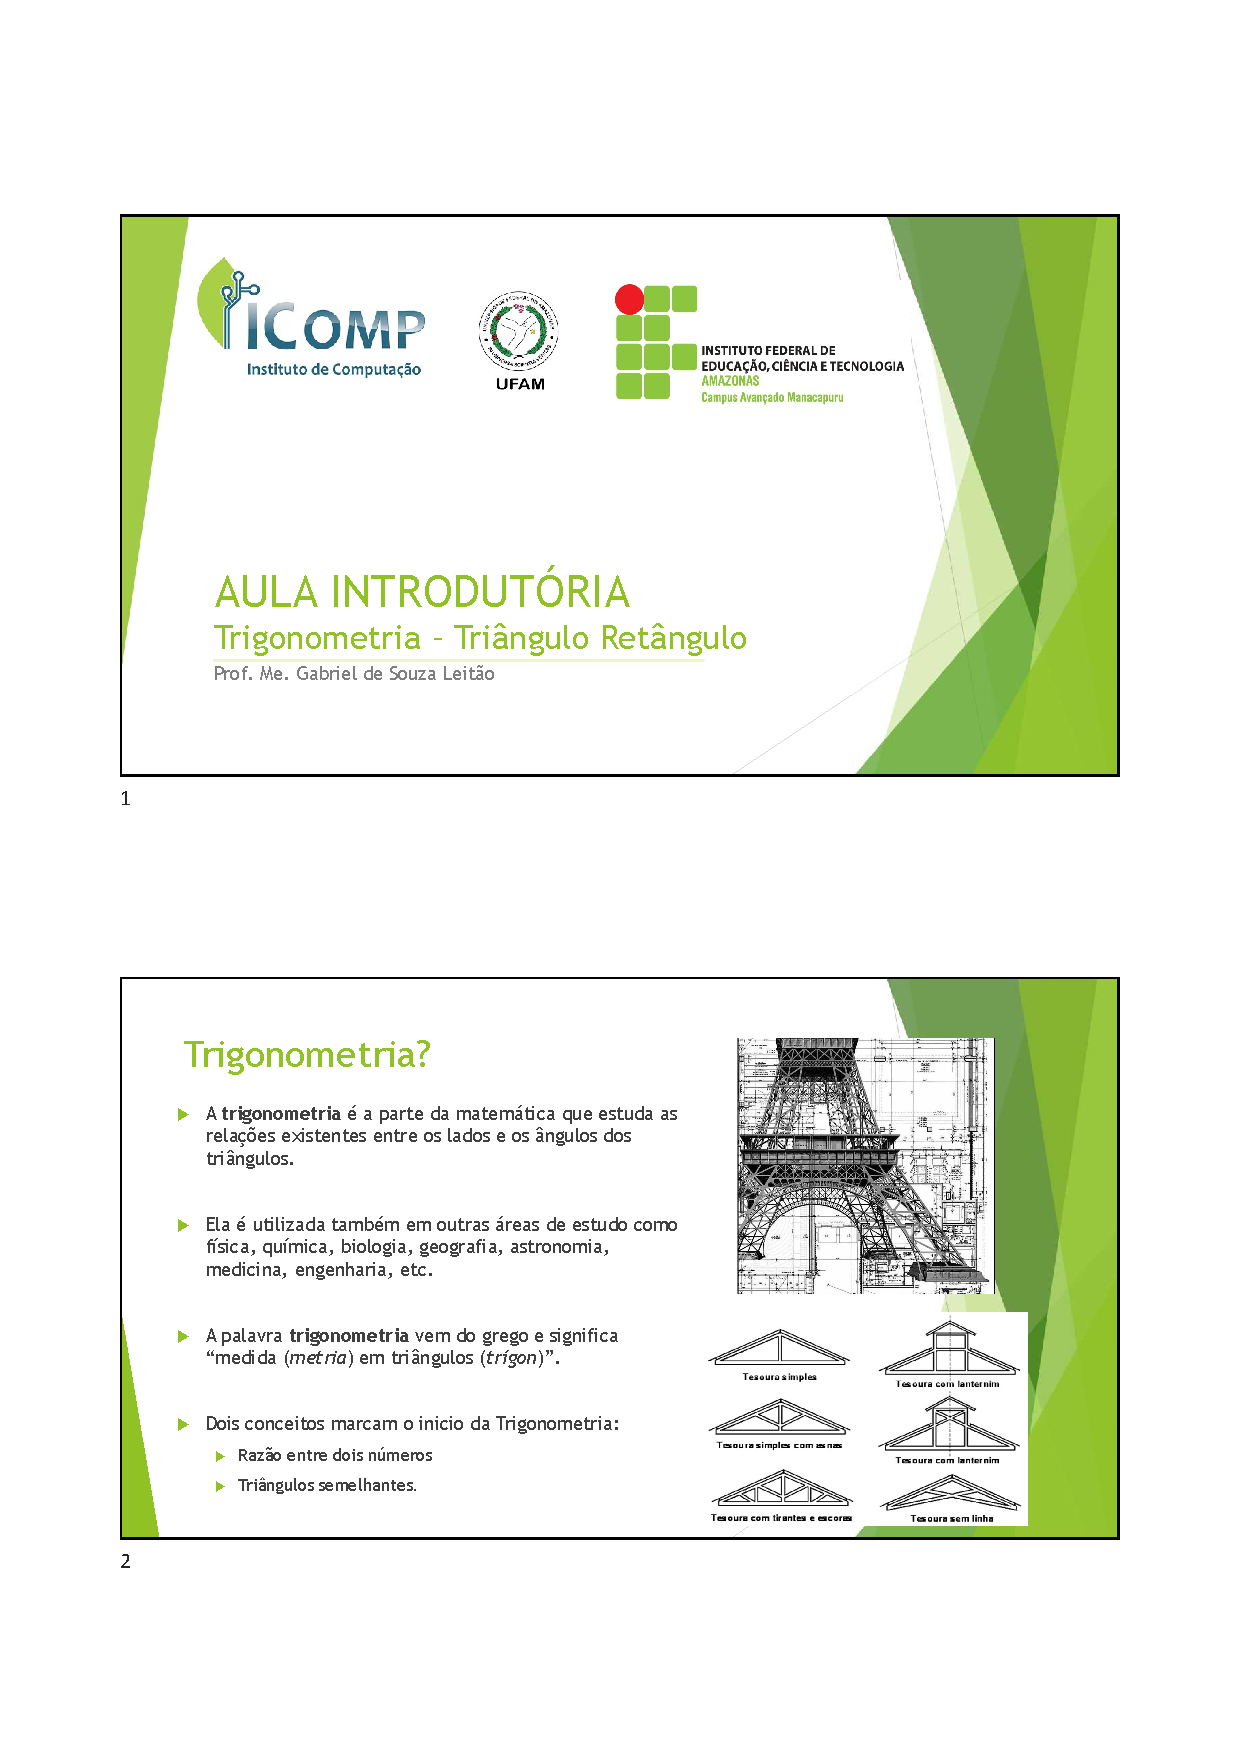
\includegraphics[width=\textwidth]{chapters/appendixLesson/Aula1Base20220611.pdf}
%\end{figure}
%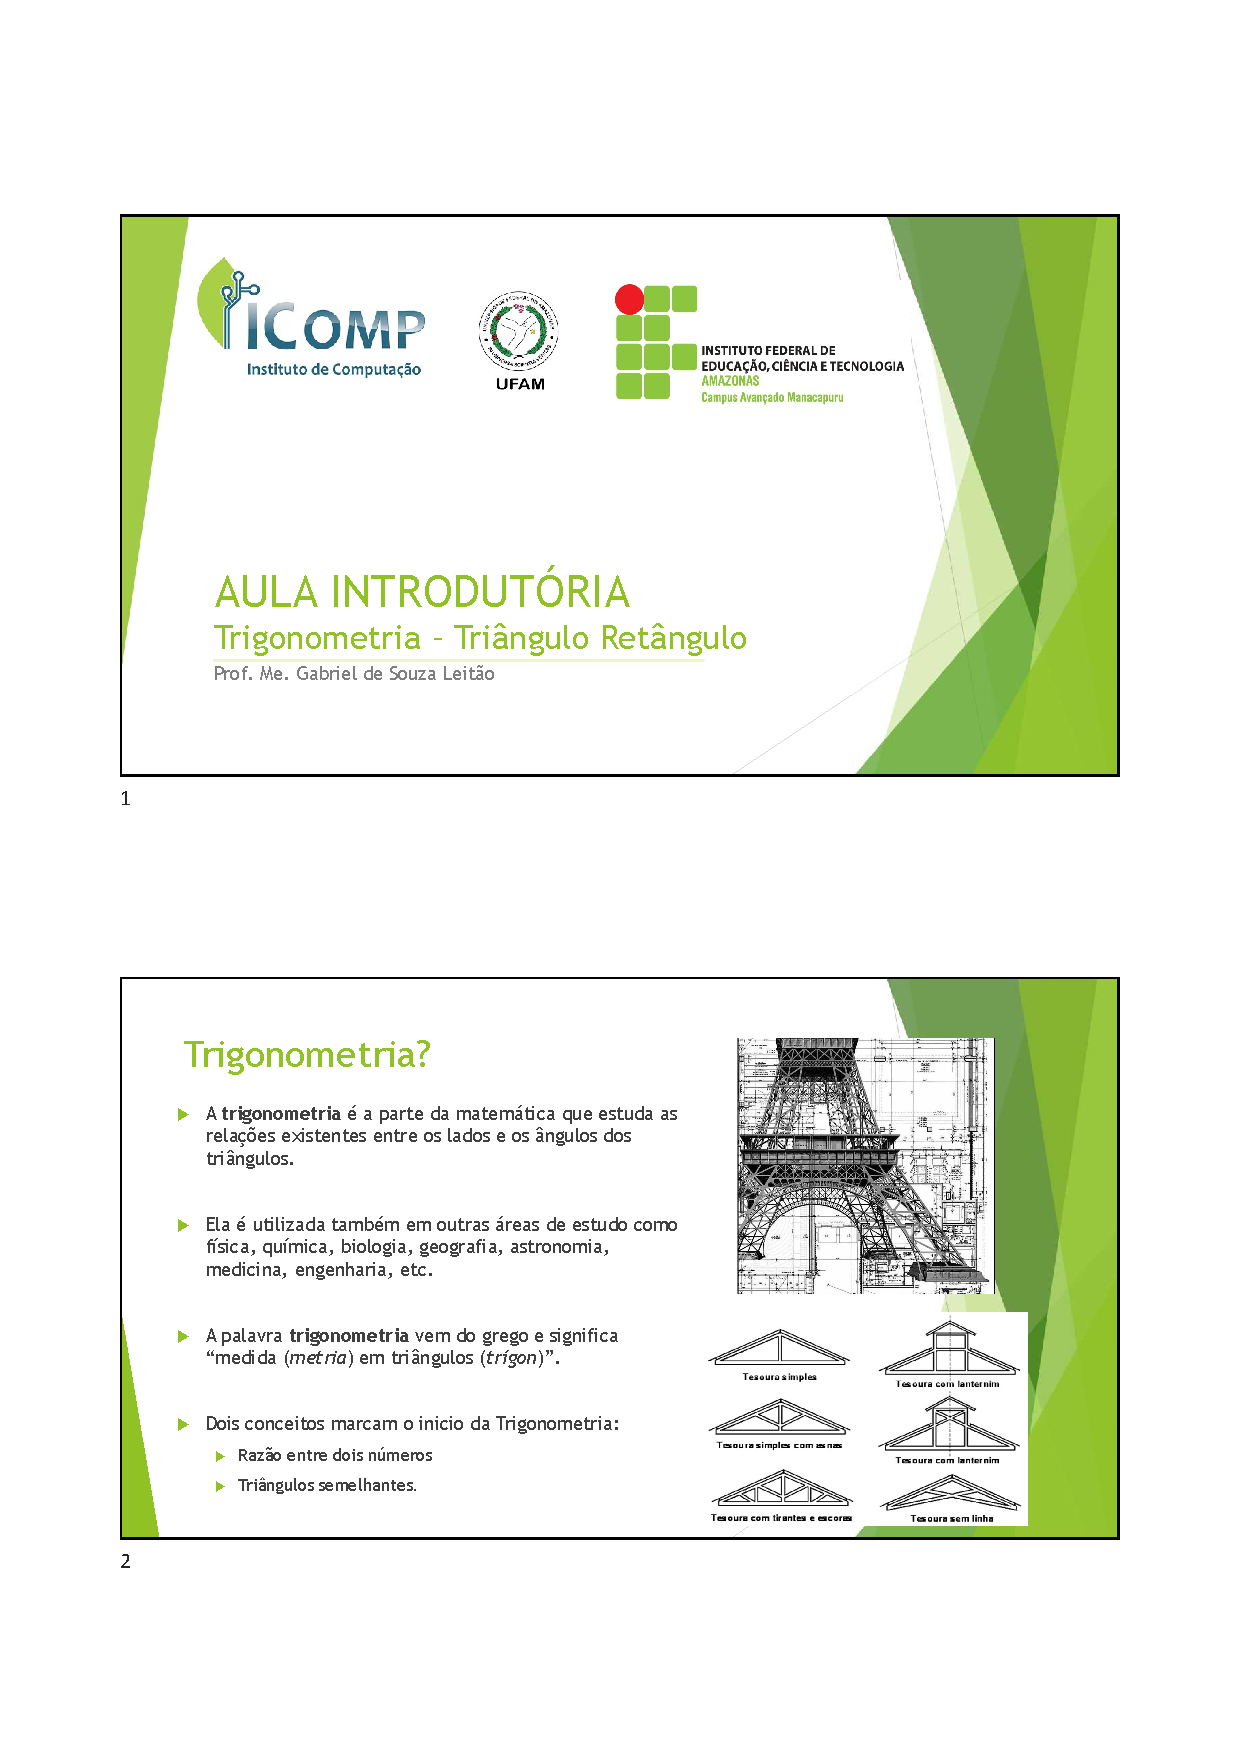
\includepdf[pages=-,offset=75 -75,pagecommand=\thispagestyle{plain}] {chapters/appendixLesson/Aula1Base20220611.pdf}
%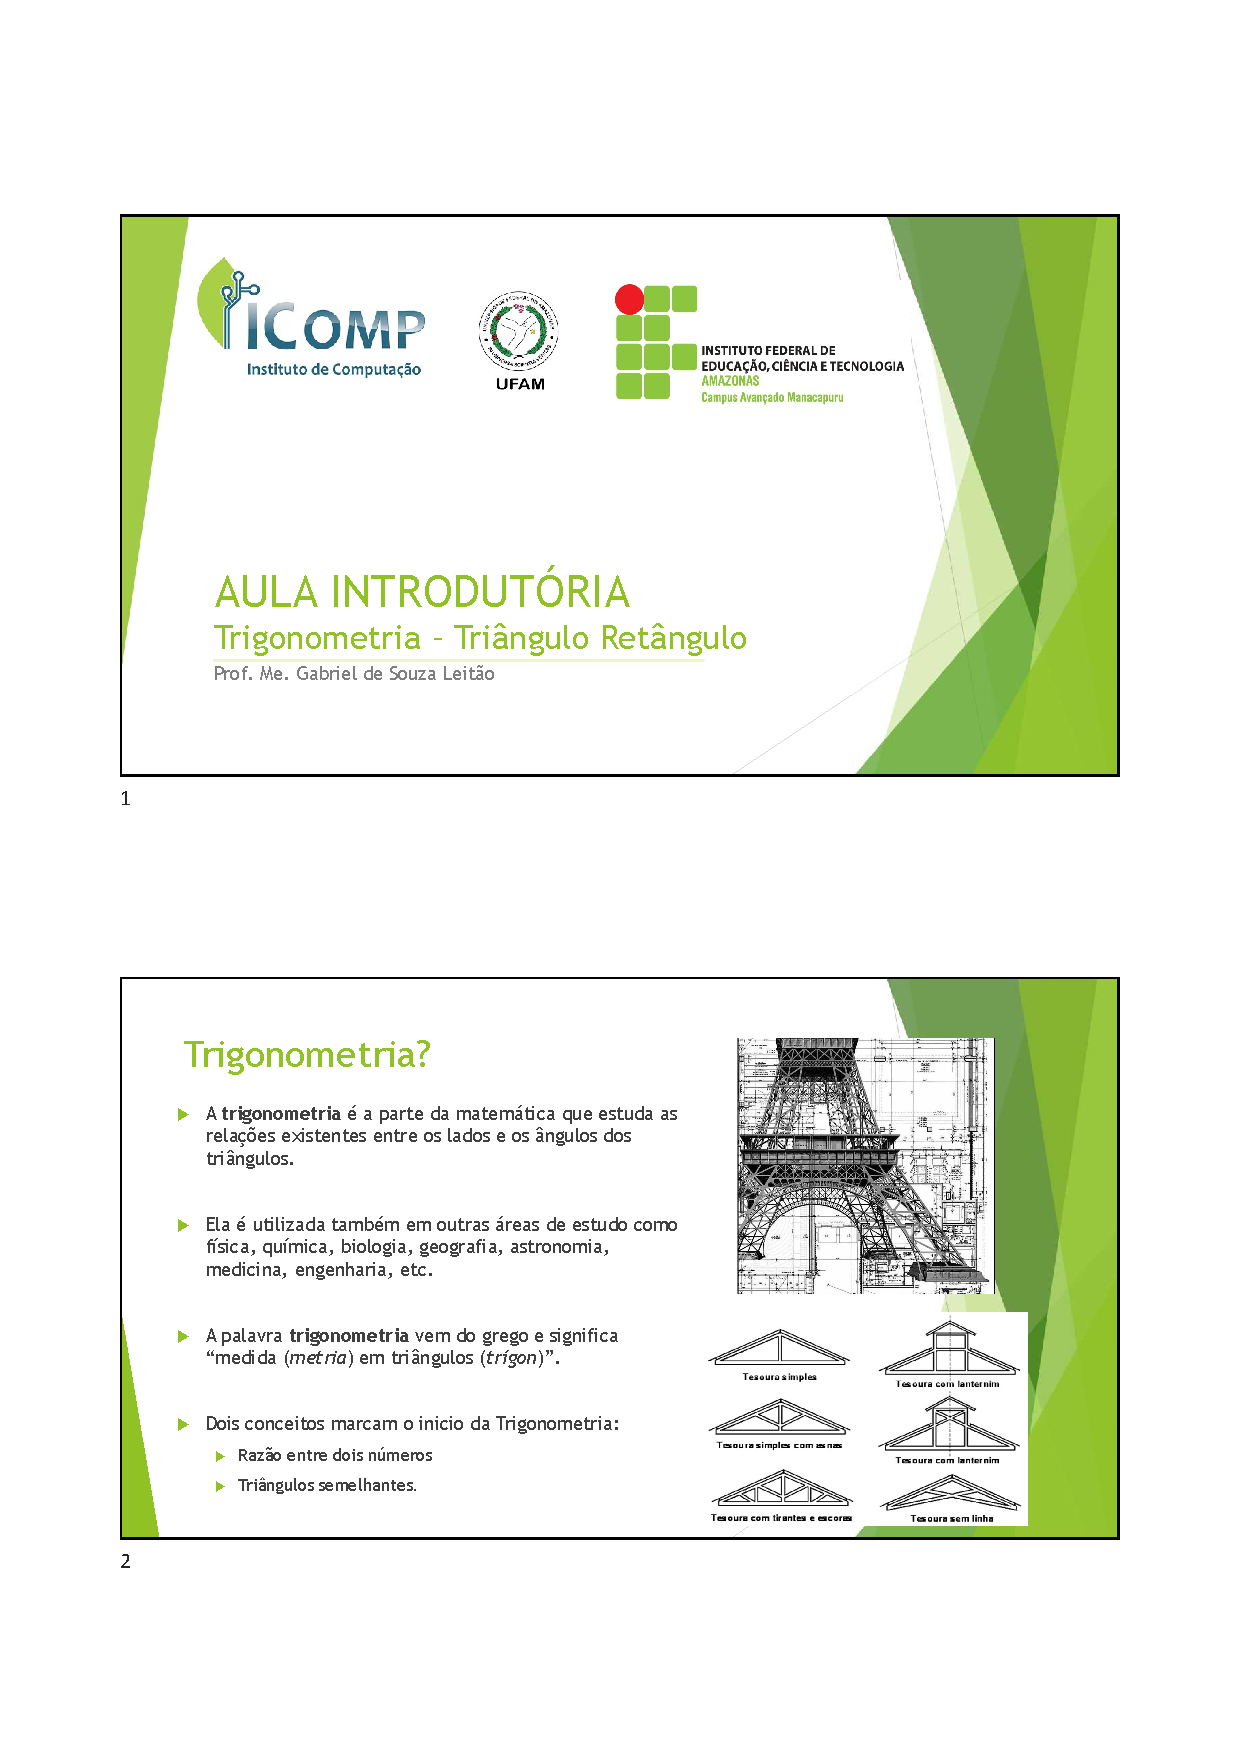
\includepdf[pages=-,pagecommand={},width=\textwidth]{chapters/appendixLesson/Aula1Base20220611.pdf}

%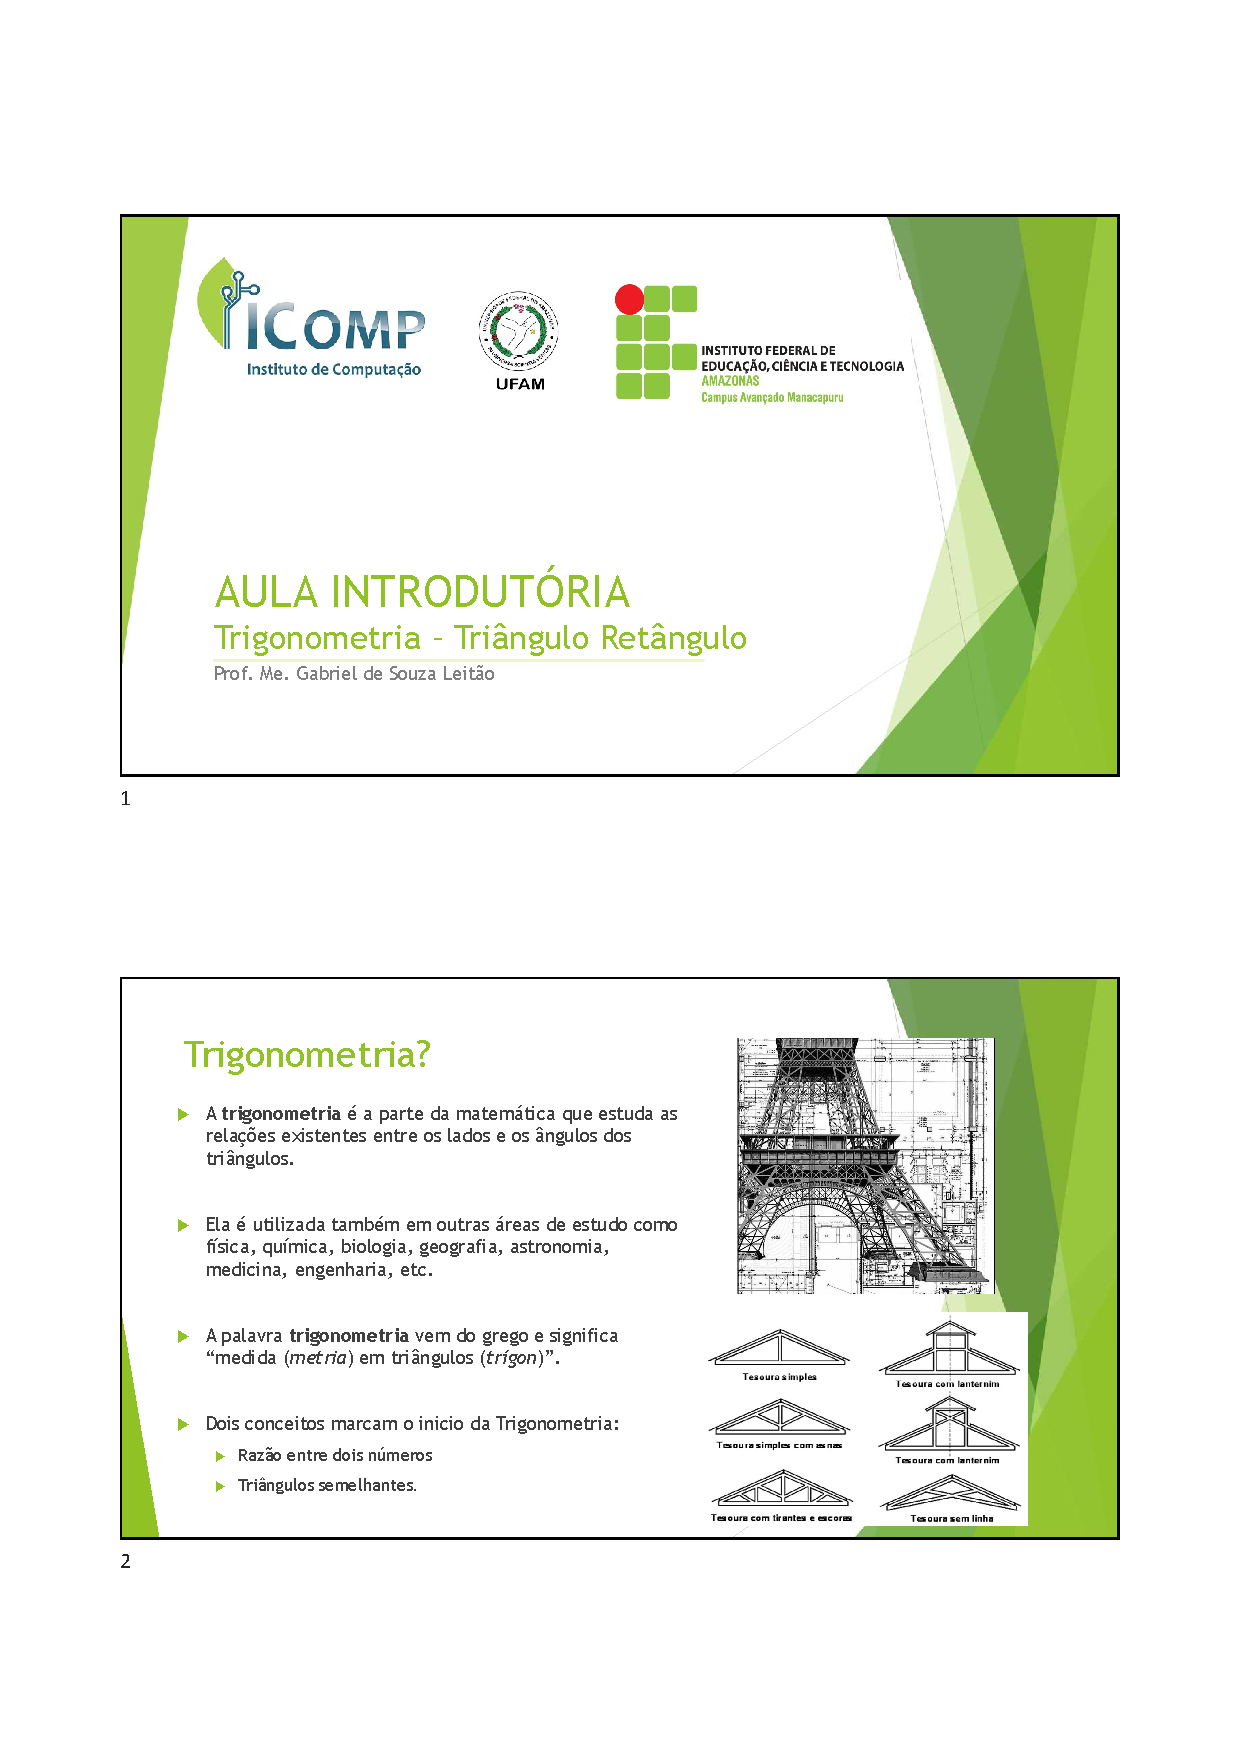
\includegraphics[scale=0.7,page=1]{chapters/appendixLesson/Aula1Base20220611.pdf}
\includegraphics[width=\textwidth,page=2]{chapters/appendixLesson/Aula1Base20220611.pdf}
\includegraphics[width=\textwidth,page=3]{chapters/appendixLesson/Aula1Base20220611.pdf}
\includegraphics[width=\textwidth,page=4]{chapters/appendixLesson/Aula1Base20220611.pdf}
\includegraphics[width=\textwidth,page=5]{chapters/appendixLesson/Aula1Base20220611.pdf}
\includegraphics[width=\textwidth,page=6]{chapters/appendixLesson/Aula1Base20220611.pdf}
\includegraphics[width=\textwidth,page=7]{chapters/appendixLesson/Aula1Base20220611.pdf}